\subsection{Comparison}
To be able see if any of the attributes have had an big effect on whether the different subjects got CHD, we plotted some of the attributes against he each other, this would also help us to spot highly unlikely data.

Some of the attributes we thought would be interesting to compare to each other, were amongst other tobacco and alcohol, since these are often considered bad for peoples health. In figure \ref{AlcoTobac} we can see those two attributes plotted against each other. Here it does look like that tobacco has an bigger influence on CHD the alcohol, but we can't really tell that much more about these two from this figure since the spread of negative and positive seems very similar.

\begin{figure}[H]
\centering
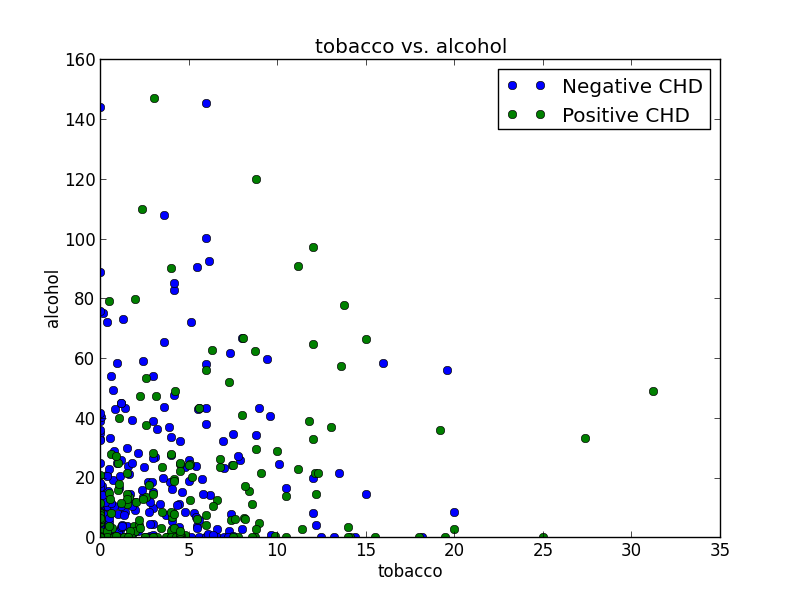
\includegraphics[width=7cm, keepaspectratio=true]{pictures/tobaccoAlcohol.png}
\vspace{-0.4cm}
\caption{\footnotesize Tobacco vs. Alcohol}
\label{AlcoTobac}
\end{figure}

Alcohol and tobacco wasn't the only attribute we thought would be interesting to look at, we also thought of what the more obese subject would look like. In the comparison figure \ref{ObeAsi} we see the adiposity and obesity put up against each other. One of the first things that catches your eyes in this, is the top left dot and the bottom right dot. These two is a bit different then the others, since they lie far from mass of subject that gathers in a bit bend line. This could be the result of wrongful data or just a bit bizarre subject. But these would be considered outliers in this comparison.

When you look at figure \ref{ObeAsi} you see the that the higher the values get the more subjects got CHD. This could say that the higher numbers a subject got in adiposity and obesity the chance there is for the subject to get CHD.

\begin{figure}[H]
\centering
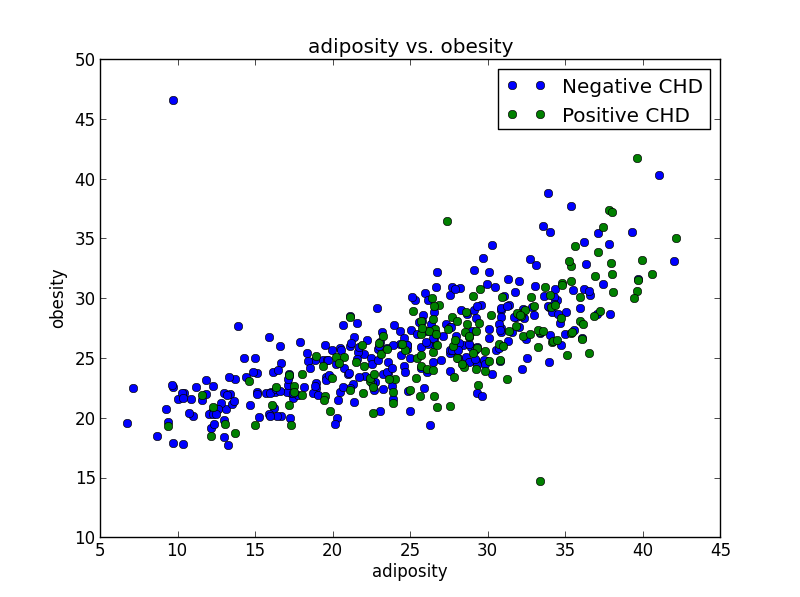
\includegraphics[width=7cm, keepaspectratio=true]{pictures/adiposityObesity.png}
\vspace{-0.4cm}
\caption{\footnotesize Adiposity vs. Obesity}
\label{ObeAsi}
\end{figure}

In figure \ref{typeAlco} we try to see if more aggressive subjects have a higher chance on getting CHD, and if alcohol would make difference in how aggressive subject would be. What we can see in the figure is at first that alcohol doesn't seem to have a big influence on how aggressive the different subject is. But it does seem the very aggressive people have an higher chance of being positive for CHD. In general i does seem like there is a similar spread in both positive and negative tested subjects.

\begin{figure}[H]
\centering
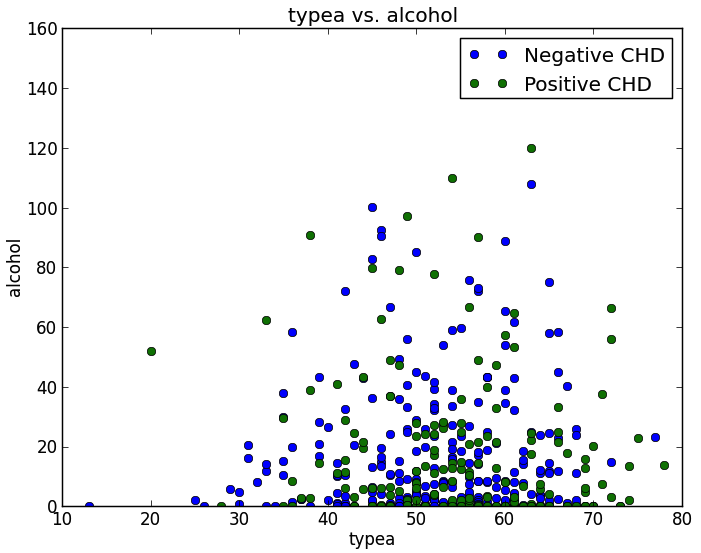
\includegraphics[width=7cm, keepaspectratio=true]{pictures/typeaalcohol.png}
\vspace{-0.4cm}
\caption{\footnotesize Type-a vs. Alcohol}
\label{typeAlco}
\end{figure}